\documentclass{article}

\usepackage{booktabs}
\usepackage{tabularx}
\usepackage{hyperref}
\usepackage[english]{babel}
\usepackage{enumitem}
\usepackage{pdflscape}
\usepackage{array}
\usepackage{longtable}
\graphicspath{ {./images/} }
\usepackage{float}
\hypersetup{
    colorlinks=true,       % false: boxed links; true: colored links
    linkcolor=red,          % color of internal links (change box color with linkbordercolor)
    citecolor=green,        % color of links to bibliography
    filecolor=magenta,      % color of file links
    urlcolor=cyan           % color of external links
}

\newcounter{srreqnum} %Likely change number
\newcommand{\lthesrreqnum}{LC\thesrreqnum}
\newcommand{\srref}[1]{SR\ref{#1}}


\title{The Pot-pulator User Manual}

\author{Aaron Billones, billonea\\Gillian Ford, fordg\\Juan Moncada, moncadaj\\Steven Ramundi, ramundis}

\date{April 5, 2022}

%% Comments

\usepackage{color}

\newif\ifcomments\commentstrue %displays comments
%\newif\ifcomments\commentsfalse %so that comments do not display

\ifcomments
\newcommand{\authornote}[3]{\textcolor{#1}{[#3 ---#2]}}
\newcommand{\todo}[1]{\textcolor{red}{[TODO: #1]}}
\else
\newcommand{\authornote}[3]{}
\newcommand{\todo}[1]{}
\fi

\newcommand{\wss}[1]{\authornote{blue}{SS}{#1}} 
\newcommand{\plt}[1]{\authornote{magenta}{TPLT}{#1}} %For explanation of the template
\newcommand{\an}[1]{\authornote{cyan}{Author}{#1}}

%% Common Parts

\newcommand{\progname}{ProgName} % PUT YOUR PROGRAM NAME HERE
\newcommand{\authname}{Team \#, Team Name
\\ Student 1 name
\\ Student 2 name
\\ Student 3 name
\\ Student 4 name} % AUTHOR NAMES                  

\usepackage{hyperref}
    \hypersetup{colorlinks=true, linkcolor=blue, citecolor=blue, filecolor=blue,
                urlcolor=blue, unicode=false}
    \urlstyle{same}
                                


\begin{document}

\maketitle
\thispagestyle{empty}

\pagenumbering{roman}

\begin{tabularx}{\textwidth}{p{3cm}p{4cm}X}
    \toprule {\bf Date} & {\bf Version} & {\bf Notes}\\
    \midrule
    2022-04-5 & Juan Moncada,& Initial release\\&Aaron Billones,\\&Steven Ramundi,\\&Gillian Ford \\
    
    \bottomrule
\end{tabularx}

~\newpage

\tableofcontents

~\newpage

\pagenumbering{arabic}

\section{Introduction}

Welcome to the user manual for the Pot-pulator - a machine designed to assist Sheridan Nurseries in populating their trays with pots, in preparation for planting with soil and seeds. The Pot-pulator is used to automate this process to reduce the need for manual labour, improving efficiency and productivity in the nursery. This manual will provide guidance on the continuous operation of the Pot-pulator, providing the information needed to effectively utilize this powerful tool.

\section{Getting started}

\subsection{Operation Steps}
When using the Pot-pulator, start by fulling the machine with trays in the tray dropper section, and empty pots in the pot dropper section. The tray dropper can hold 30 trays, while the pot dropper can hold up to 300 pots, requiring refills every 15 minutes. Within this time, the machine requires no further action from the user once the on button has been pressed. Under normal operation, the Pot-pulator will follow the steps below:
\\
\\ \noindent 1.	Fill the machine with empty pots and trays\\ 
\noindent 2.	Press the "on" button

 \noindent 3.	Tray dropper will dispense trays one at a time

 \noindent 4.	A tray will drop onto the conveyer belt and move to the next section

 \noindent 5.	Conveyer positions the tray to prepare for pot dropping

 \noindent 6.	Conveyer stops and drops 2 pots at a time into the tray

 \noindent 7.	Conveyer continues to move to the next available slots in the tray, until the entire tray is filled with pots (10 pots)

 \noindent 8.	The verification subsystem will determine if all the pots have been placed correctly in the tray, outputting an LED when a pot is missing or out of place. 
\\
\\ \noindent Throughout the operation of the device, the user interface will display the current status of the machine. To learn more about the user interface and how to navigate it, please refer to the "User Interface" section of this manual.
\subsection{Safety and Precautions}
When refilling pots and trays, ensure that the machine is turned off. Once they have been loaded into the system, the user can then turn on the machine for operation.
\section{User Interface}
\begin{figure}[H]
    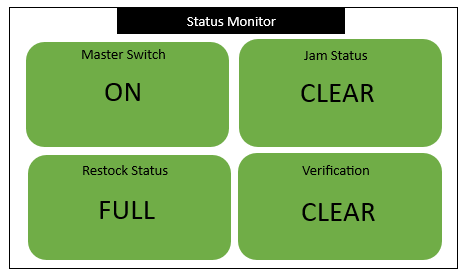
\includegraphics{statusgood.png}
    \caption{System Context Diagram}
    \label{fig:scope}
  \end{figure}
The user interface includes a screen with the output functions of the machine. The user does not have to interact with this device, as it is only used to provide information on the status of the Pot-pulator.
\subsection{Power Switch Status}
This section informs the user if the machine is on or off.
\subsection{Pot Missing}
This section informs the user if there is a pot missing or out of place once the trays reach the verification system.
\subsection{Tray Jam}
This section informs the user that there is a jam in the stack of trays in the tray dropper. This will require the machine to be turned off and the trays to be taken out and restacked. 
\subsection{Pot Jam}
This section informs the user that there is a jam in the stack of pots in the pot dropper. This will require the machine to be turned off and the pots to be taken out and restacked. 
\subsection{Pot Dispenser Empty}
This section informs the user that the pot dispenser is empty. The user will need to refill the pot dropper every 15 minutes.
\subsection{Tray Dispenser Empty}
This section informs the user that the tray dispenser is empty. The user will need to refill the tray dropper every 15 minutes.
\section{Features and Functionality}
\subsection{Conveyer}
The user can start the Pot-pulator by pressing the on switch on the conveyer belt. The conveyer will then move the trays through each system, starting and stopping based on the position they need to be in for pot dispensing. 
\subsection{Tray Dispenser}
Up to 30 trays can be manually inserted to the top of the tray dispenser at the start of the system. The user will need to refill the tray dispenser every 15 minutes.
\subsection{Pot Dropper}
Up to 300 pots can be manually inserted to the top of the pot dropper at the start of the system. The user will need to refill the pot dropper every 15 minutes. There are two sections in the pot dropper where pots can be inserted, and they should be stacked and placed into both equally.
\subsection{Verification System}
The verification system will notify the user when there is a problem with the system. If there is a pot missing or out of place, an LED will light up, alerting the user that the system is not functioning as intended. 
\section{Troubleshooting and FAQs}
\subsection{What happens if trays get stuck?}
If the trays get stuck, turn off the machine and remove them from the stack, and refill them normally. Once they are in place, turn the machine on to run as normal.
\subsection{What happens if pots get stuck?}
If the pots get stuck, turn off the machine and remove them from the stack, and refill them normally. Once they are in place, turn the machine on to run as normal.
\subsection{How many trays can the tray dropper hold?}
The tray dropper can hold up to 30 trays, but it will need to be refilled every 15 minutes.
\subsection{How many pots can the pot dropper hold?}
The pot dropper can hold up to 300 pots, but it will need to be refilled every 15 minutes.
\subsection{How does the Pot-pulator verify that all the pots have been placed correctly in the tray?}
The verification subsystem will determine if all the pots have been placed correctly in the tray, outputting an LED when a pot is missing or out of place.
\subsection{How do I refill the Pot-pulator with trays and pots?}
When refilling pots and trays, ensure that the machine is turned off. Once they have been loaded into the system, the user can then turn on the machine for operation.
\subsection{How can I use the user interface of the Pot-pulator?}
The user interface will display the current status of the machine. To learn more about the user interface and how to navigate it, please refer to the "User Interface" section of the manual.

\end{document}